%!TEX root = ../docu.tex
\section{Entwicklung}

\subsection{Benutzeroberfläche}

Die Interaktion von Benutzer und Programmstrukturen erfolgt über eine Benutzeroberfläche oder auch GUI\footnote{engl. Graphical User Interface}. Diese ist besonders einfach gehalten, um eine intuitive Bedienung des Programms zu gewährleisten.

\begin{figure}[h!t]
\begin{center}
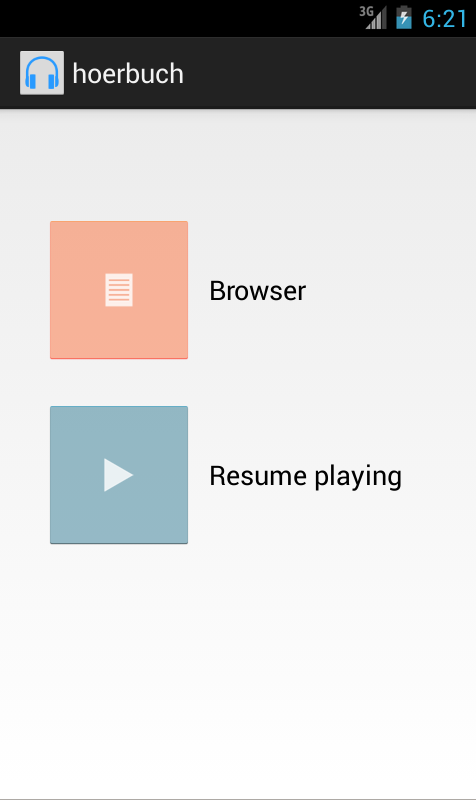
\includegraphics[scale=.2]{images/mainscreen}
\caption{Hauptansicht der Anwendung}
\label{mainscreen}
\end{center}
\end{figure}

Position und Größe von Elementen und Bedienstrukturen sind so gewählt, dass die Eingabe über das Display so einfach wie möglich ist. Über eine Hauptansicht gelangt der Benutzer zu allen benötigten Funktionen der Anwendung. Diese Ansicht ist in Abbildung \ref{mainscreen} dargestellt.

Die Farbgebung orientiert sich am Holo-Design von Android. Dieses Design wird durch klare Farbgebung in Schwarz und Blau charakterisiert. Die Hauptfunktionen beinhalten zum einen die Auswahl einer bestimmten Audiodatei und zum anderen das Wiederaufnehmen von abgebrochenen Wiedergaben. Beide Funktionen werden über durchlaufbare Listen dargestellt und variieren nur minimal vom Design. Dennoch sind es zwei unterschiedliche Funktionen.

\begin{figure}[h!t]
\begin{center}
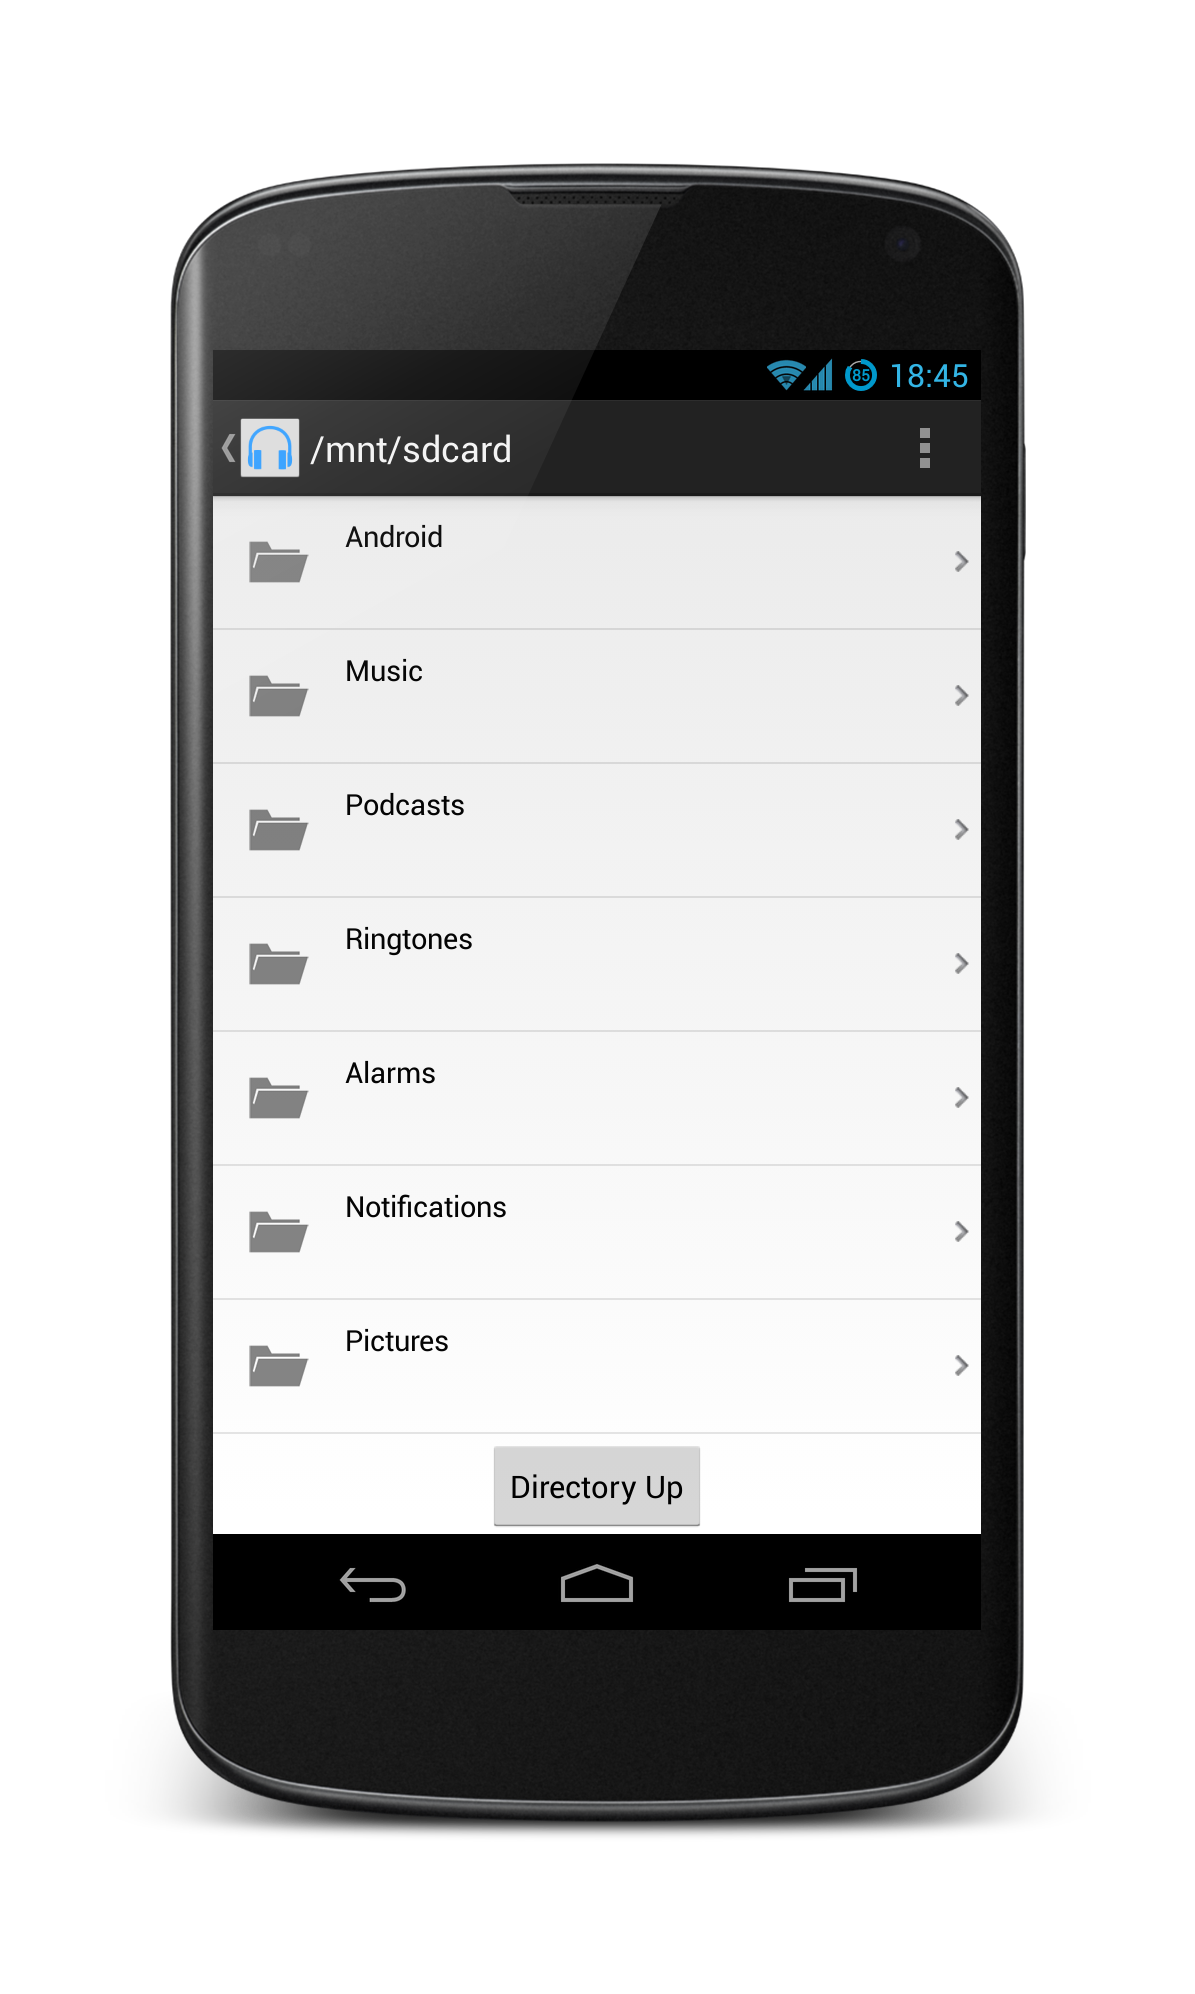
\includegraphics[scale=.2]{images/browsing}
\caption{Auswahl der Audiodatei durch Liste}
\label{browsing}
\end{center}
\end{figure}

Abbildung \ref{browsing} zeigt die Auswahlmöglichkeit über die Listenansicht. In Abbildung \ref{broken} ist die Liste mit den abgebrochenen Wiedergaben zu erkennen.

\begin{figure}[h!t]
\begin{center}
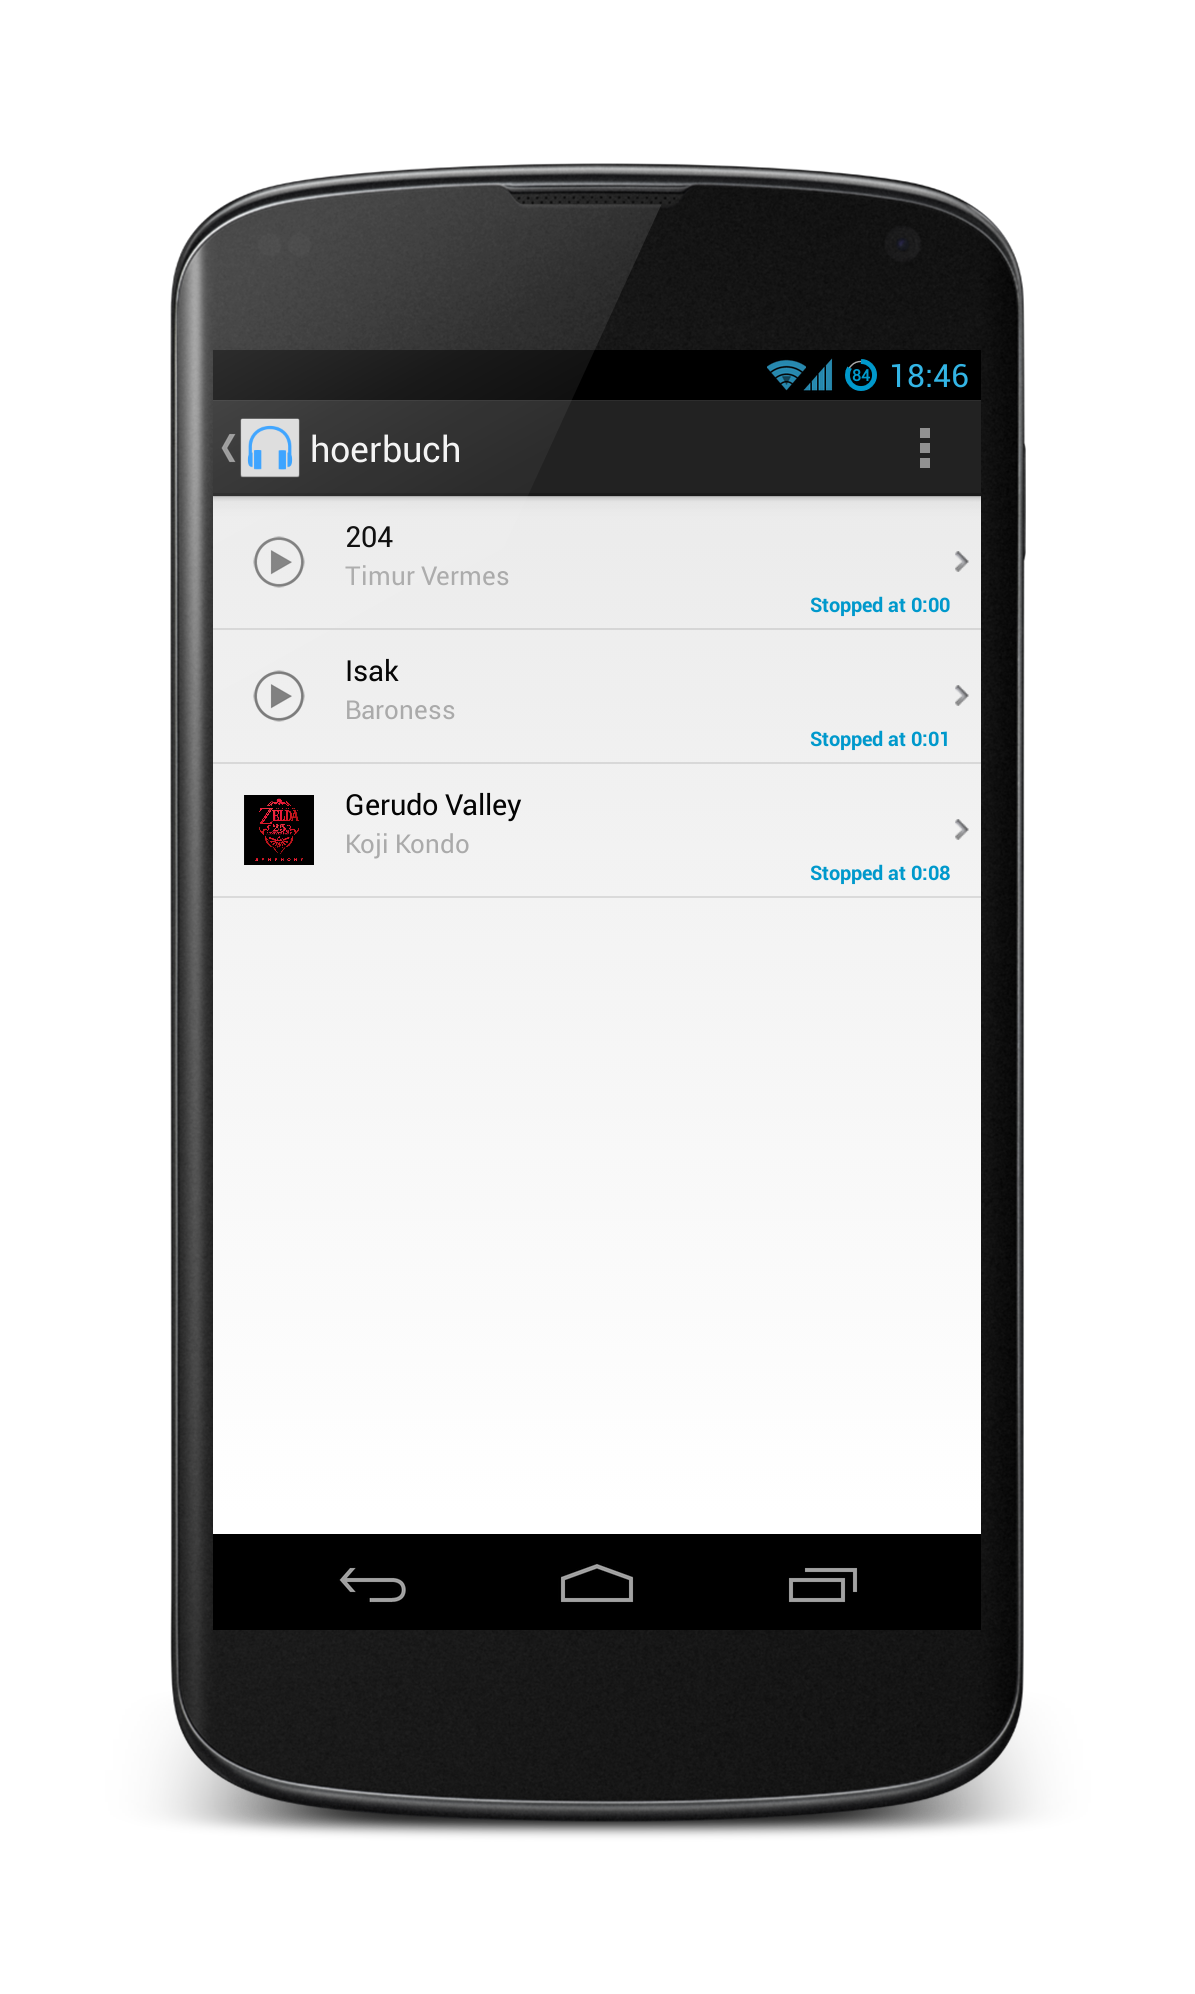
\includegraphics[scale=.2]{images/broken}
\caption{Liste mit abgebrochenen Wiedergaben}
\label{broken}
\end{center}
\end{figure}

Das Auswählen der Audiodateien erfolgt über einfache Eingaben über das Display mit Druck auf das jeweilige Element in der Liste.

Die Einstellung der Anwendung wird über die \textit{Menü}-Taste am oberen Bildschirmrand aufgerufen. Alle Funktionen bilden eigene Strukturen und sind durch separate Klassen definiert. Diese Struktur soll in den nachfolgenden Unterkapiteln von \ref{classes} behandelt werden.

\subsection{Klassenstruktur}
\label{classes}

Um ein Gesamtbild über die Struktur des Projektes zu geben, werden im folgenden Abschnitt die Klassen vorgestellt und zusammengefasst, die eine wichtige Funktion in der Anwendung übernehmen.

\subsubsection{Activities}

Als erstes werden in Abbildung \ref{cd_activities} die Activities vorgestellt. Wie in Abschnitt \ref{components} beschrieben, stellen Activities die sichtbaren Bildschirminhalte dar. Methoden die Android standardmäßig benötigt und durch das Interface \verb+Activity+ bereitgestellt werden sind einmal \verb+onCreate()+ die aufgerufen wird, wenn die Activity gestartet wurde. Weiterhin sind \verb+onCreateOptionsMenu()+, was für die Darstellung des Optionsmenüs notwendig ist, und \verb+onOptionsItemSelected()+, welches Aktionen für die Optionen definiert, in jeder Activity enthalten.

\begin{figure}[ht!]
\begin{center}
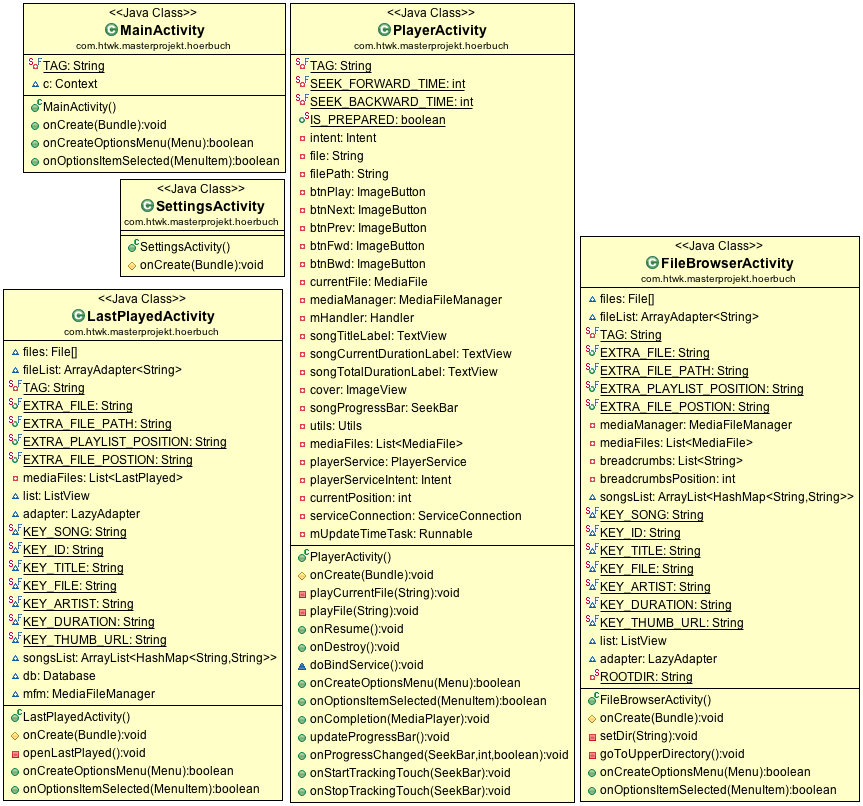
\includegraphics[scale=.5]{images/diagram}
\caption{Klassenübersicht der Activities}
\label{cd_activities}
\end{center}
\end{figure}

Die Activities selbst haben dabei folgende Aufgaben:

\begin{description}[style=nextline]
	\item[MainActivity] Wird angezeigt, wenn die Applikation gestartet wird. Außer den beiden Buttons für das Starten der \verb+FileBrowserActivity+ und der \verb+LastPlayedActivity+ befindet sich darauf nichts.
	\item[SettingsActivity] Stellt das Einstellungsmenü dar. Da die Inhalte dieses Menüs an anderer Stelle per XML definiert werden, befinden sich keine weiteren Methoden in der Klasse.
	\item[FileBrowserActivity] Wird angezeigt, wenn man auf den \emph{Browser}-Button im Hauptmenü klickt. Hier wird der Dateibrowser angezeigt, über den die Hauptnavigation durch die Hörbücher und Ordner möglich ist.
	\item[LastPlayedActivity] Stellt den Browser dar, der die letzten gehörten Hörbücher anzeigt. Man kommt in diese Ansicht, wenn man im Hauptmenü den entsprechenden Button drückt.
	\item[PlayerActivity] Der eigentliche Hörbuch-Player. Dieser wird gestartet, wenn man eine Datei im Browser ausgewählt hat.
\end{description}

\subsubsection{Die MediaPlayer-Architektur}

\begin{figure}[ht!]
\begin{center}
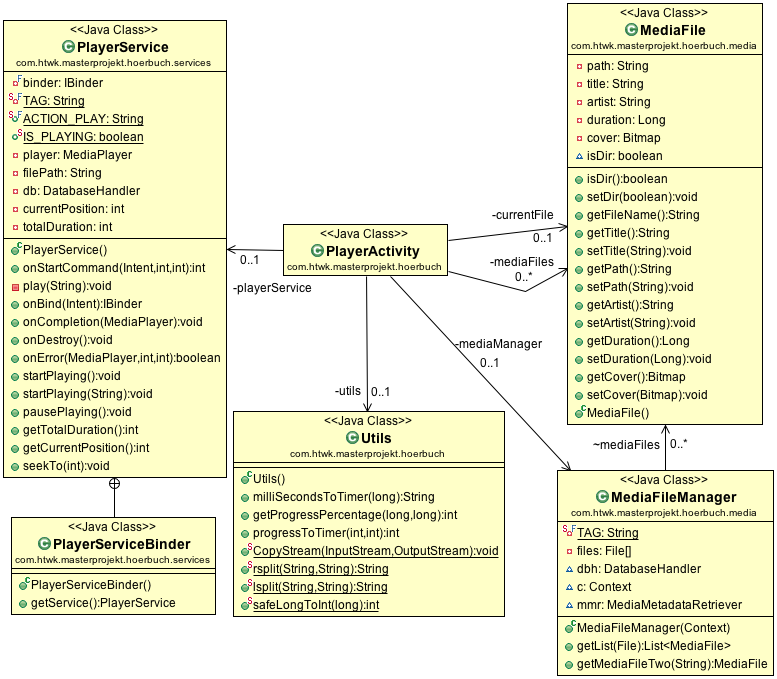
\includegraphics[scale=.5]{images/cd_media}
\caption{Klassenübersicht der MediaPlayer-Architektur}
\label{cd_media}
\end{center}
\end{figure}

Um Mediadateien abspielen zu können, stellt die Android-Plattform die Klasse \verb+MediaPlayer+ zur Verfügung. Um ein Hörbuch abzuspielen, wird die gewählte Datei geladen und vorbereitet. Das übernimmt der \verb+PlayerService+. Die Entscheidung, dies in einen Service, einen gesonderten Thread auszulagern ist damit begründbar, dass das vorbereiten der Datei bei großen Datein den Haupt-Thread, in dem das User-Interface läuft, blockiert und die Anwendung träge macht. Gerade im Bereich der Hörbücher muss der Player mit Dateien bis zu \SI{1}{GB} zurechtkommen. Durch die Auslagerung in den Service kann das Hörbuch im Hintergrund vorbereitet werden, ohne, dass der Nutzer eine Verzögerung der Oberfläche mitbekommt.

Wie in Abbildung \ref{cd_media} zu sehen, bildet die \verb+PlayerActivity+ das Zentrum.Ausgehend davon befindet sich der \verb+PlayerService+ und der \verb+PlayerServiceBinder+ welcher die Kommunikation zwischen dem Service und der Activity unterstützt.

Um eine Mediendatei ausreichend gut zu repräsentieren, wurde die Datenstruktur \verb+MediaFile+ implementiert. Diese enthält alle Daten, die für den Player zum Abspielen oder zur Darstellung von Informationen notwendig sind. 

Der \verb+MediaFileManager+ hat die Aufgabe Dateien vom Speicher zu lesen. Dabei extrahiert er dessen Metainformationen und speichert diese zusammen mit dem Pfad als Liste von \verb+MediaFile+. Diese Liste kann vom Browser oder vom Player als Playlist verwendet werden. Damit nur Dateien gelesen werden, die auch wirklich abgespielt werden können, wird der \verb+AudioFilter+ verwendet. Dieser filtert vorher definierte Dateitypen und vermeidet unnötiges Lesen von nicht abspielbaren Dateien.

Die Klasse \verb+Utils+ bietet verschiedene Werkzeuge an, die unter anderem für die Darstellung notwendig sind. So können damit beispielsweise die vom MediaPlayer ausgegebenen Millisekunden in ein lesbares Format umgewandelt werden.

\subsection{Einstellungen}

Das Einstellungsmenü soll in jedem Zustand der Applikation erreichbar sein. Um dies zu ermöglichen, gab es bis Android-Version 2.3 eine separate Menütaste auf den Geräten. Diese wurde mit der Einführung von Android 4.0 abgeschafft. Um dennoch ein Menü aufrufen zu können, wird ein Button, der auf dem Bildschirm nur bei Bedarf dargestellt wird, verwendet.

Drückt ein Benutzer den Menü-Button, welcher sich meistens am oberen Bildschirmrand befindet und durch drei übereinanderliegende Punkte dargestellt ist, öffnet sich das Dropdown-Menu. Dieses wird durch den Entwickler mit Einträgen befüllt und kann dadurch bestimmte Funktionen bereitstellen. Eine typische Funktion ist die Einstellungsseite.

Die Konfiguration der Einstellungsmöglichkeiten, welche dem Nutzer zur Verfügung gestellt wird, erfolgt über eine XML Datei. In älteren API-Versionen wurde dies noch durch Klassen realisiert. Diese Klassen und Methode sind in den Version ab Android Version 4 veraltet und sollten nicht mehr verwendet werden. Die erwähnte XML-Datei wird nun durch bestimmte Regler und Kontrollstrukturen bestückt. Diese Strukturen werden durch ID's validiert. Ihre Werte können durch eine Abfrage aus der Anwendung heraus ausgelesen werden. Sollten keine geeigneten vorgefertigte Kontrollstrukturen, wie zum Beispiel Radio-Button oder Checkboxen vorhanden sein, so können eigene Strukturen eingebettet werden.

Im konkreten Projekt existiert keine Struktur für das Speichern und Durchsuchen eines Ordnerpfades. Dieser \textit{FilePicker} wurde daher geziehlt implementiert und kann aus dem Einstellungsmenü aufgerufen werden.

\begin{center}
\begin{figure}
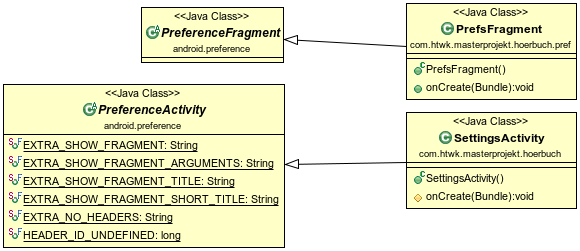
\includegraphics[scale=0.7]{images/settings}
\caption{Klassen für die Implementierung der Einstellungen}
\label{settings}
\end{figure}
\end{center}

Wurde der gewünschte Ordner gefunden, kann dieser in den Einstellungen gespeichert werden. Alle anderen Komponenten der Anwendung können nun auf diese Einstellungen zugreifen. Dies wird über den \textit{PreferenceManager} realisiert. Er benötigt für die Abfrage des Wertes lediglich die ID der Einstellung. Die angesprochene ID hat einen Wert hinterlegt welche bei der Abfrage zurückgegeben wird. Zur Sicherheit wird bei der Abfrage ein Standartwert angegeben, im Falle, dass die Einstellung nicht gefunden oder ausgelesen werden konnte. Die einmal eingetragen Einstellungen sind jederzeit abrufbar und auch nach Beenden der Applikation immer noch vorhanden.

Die Abbildung \ref{settings} zeigt die benötigten Klassen für die Implementierung der Funktionalität der Einstellungen.

\subsection{Datenbank}

\subsubsection{Grundlagen}

Das Android eine Schnittstelle für SQlite Datenbanken anbietet, wurde schon in einem vorherigen Abschnitt \ref{Datenbankstrukturen} behandelt. Anschließend wird nun erläutert, wie man diese Anbindung benutzt und wie Daten gespeichert und abgefragt werden.

Zunächst benötigen wir eine Klasse welche die API-Klasse \textit{SQLiteOpenHelper} erweitert. Diese bildet nun die Schnittstelle unserer Applikation und der Datenbank, welche wir benutzen möchten bzw. anlegen möchten.

Jeder Applikation ist es möglich, mehrere Datenbanken anzulegen und zu verwenden. Um Datenbanken voneinander unterscheiden zu können, werden die einzelnen Datenbanken über Namen verifiziert und aufgerufen.

Um Android mitzuteilen, welche Datenbank wir öffnen möchten, wird dem Betriebssystem mitgeteilt, um welche Applikation es sich handelt und wie der Name der zu öffnenden Datenbank ist.

Das Resultat ist eine Verbindung zu einer SQlite Datenbank. Um Daten zu speichern, wird eine Tabelle angesprochen. Diese Tabelle wir bei der Erstellung der Datenbank mit angelegabert.

Für diesen Zweck legen wir eine Methode mit den Namen \textit{onCreate} an. Diese Methode wird beim Erstellen der Datenbank ausgeführt und enthält alle SQL-Befehle zum Anlegen der von uns gewünschten Tabellen.

Sollte sich das Datenbankschema ändern, wird dies über eine weiter Variable, welche wir dem Betriebssystem mitteilen, realisiert. Eine Datenbankversion beschreibt den Stand der Datenbankstruktur. Sollte sich die Datenbankstruktur geändert haben wird die Versionsnummer erhöht und eine andere Methode wird beim Anbinden zur Datenbank aufgerufen.

\begin{figure}
\begin{center}
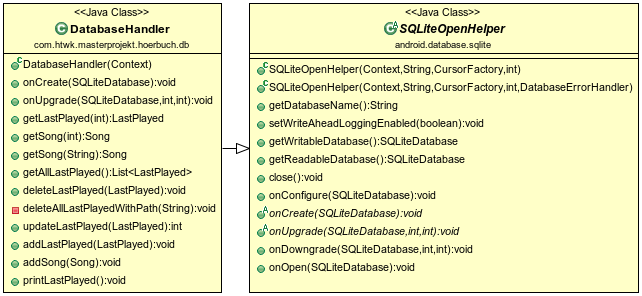
\includegraphics[scale=0.7]{images/database}
\caption{Klassen für die Implementierung der Datenbank}
\label{database}
\end{center}
\end{figure}

Diese Methode nennt sich \textit{onUpgrade} und wird bei eben erwähnter Erhöhung der Versionsnummer automatisch ausgeführt. In dieser Methode wird eine Datenmigration durchgeführt oder alle bestehenden Daten gelöscht und neue Tabellen angelegt.

Durch diesen Mechanismus ist die Aktualität des Datenbanklayouts immer gegeben. In der Abbildung \ref{database} sind die Klassen ersichtlich, die es ermöglichen mit der Datenbank zu kommunizieren. Für die Verwendung der Daten ist es ratsam Objekte zu verwenden, um abgefragte Datensätze weiter zu verwenden. Ein solches Objekt wird in Abbildung \ref{dbmodel} dargestellt.

\begin{figure}
\begin{center}
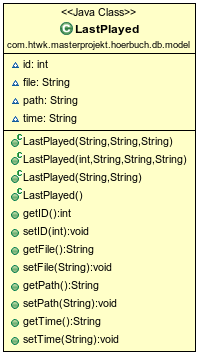
\includegraphics[scale=0.7]{images/dbmodel}
\caption{Obejkt zum transport der datensätze}
\label{dbmodel}
\end{center}
\end{figure}

\subsubsection{Abfragen}

Eine Datenbankabfrage wird über einen SQL-Befehl an die Datenbank gestellt. Mit dem Befehl \textit{SELECT} und der Angabe der Tabelle können Daten aus der Datenbank abgefragt werden. Die Abfrage wird dafür in eins Cursor-Objekt geladen und der Cursor anschließend zur Ausführung an die Datenbank gesendet.

Das Cursor-Objekt enthält anschließend alle abgefragten Daten, welche die Datenbank zum übergeben SQL-Befehl gefunden hat. Eine direkte Abfrage ist nicht möglich.

Es muss immer eine Cursor-Objekt verwendet werden. Möchte man nur bestimmte Daten oder zielgerichtet Datensätze aus der Datenbank laden, wird dem Cursor-Objekt eine Filterung mitgeteilt, welche von der Datenbank bei der Abfrage der Daten berücksichtigt wird.

Das Cursor-Objekt enthält eine Liste von allen Dateneinträgen die gefunden wurden. Sind mehre Datensätze gefunden wurden, können diese durchlaufen werden und jeder Datensatz einzeilig betrachtet und verarbeitet werden.

Bei der Abfrage der einzelnen Felder des Datensatzes ist es nötig, den Datentyp der einzelnen Daten zu kennen. Das Cursor-Objekt hat verschiedene Methoden, um unterschiedliche Datentypen aus den Feldern zu lesen. Diese Typen können, wie schon erwähnt, nicht typsicher abgefragt werden. So ist es möglich, ein Datenfeld des Types \textit{Integer} in eine Variable des Typen \textit{String} zu laden.

Der Zugriff zur Datenbank ist seriell und kann nur entweder lesend oder schreibend gewährleistet werden. Eine Kombination beider Vorgänge parallel ist nicht möglich. Möchte man Schreiben und Lesen, wird dies durch einen schreibenden Zugriff und einen anschließenen lesenden Zugriff realisiert. Diese beiden Vorgänge müssen separat initiiert werden.

\subsubsection{Löschen}

Das Löschen von Daten erfolgt ebenso wie das Selektieren durch SQL-Befehle. Anders, als bei dem Selektieren existiert hierfür kein Cursor-Objekt. Es wird lediglich mitgeteilt, welcher Datensatz in welcher Tabelle gelöscht werden soll.

\subsubsection{Ändern}

Ähnlich verhält es sich mit den Ändern von Datensätzen. Hierfür wird der Datenbank mitgeteilt, welcher Datensatz geändert werden soll und welche Datenfelder mit welchem Wert gesetzt werden soll.

Die Referenzierung einzelner Datensätze erfolgt über Primärschaltregler oder andere Datenfelder, welche im SQL-Befehl angegeben werden müssen.

\subsubsection{Einfügen}

Das Anlegen neuer Datensätze wird durch die Methode \textit{insert} ausgelöst. Diese Methode verlangt ein Liste von Schlüssel-Wert-Paaren, um einen Datensatz anlegen zu können.

Die Liste von Paaren repräsentiert den eigentlichen Datensatz. In ihr werden alle Datenfelder und die dazugehörigen Werte abgelegt. Ausgeschlossen ist der Primärschlüssel. Dieser wird durch einen Trigger in der Datenbank automatisch erzeugt und beim Einfügen in die Datenbank an den Datensatz angehangen und gespeichert. Der Methode wird nun die Liste mit den Daten übergeben und die Tabelle genannt, in der die Daten abgelegt werden soll. Der Trigger muss nicht separat angelegt werden, sondern wird durch das Erzeugen einer Spalte, welche als Primärschlüssel gekennzeichnet wird, angelegt.